\chapter{Complete Example}

To illustrate our concept, we use a language transformation scenario: Suppose we have a model representing the abstract syntax graph (ASG) of a program. The ASG is language-specific, of course. If we want to generate code from the ASG for a target language other than the language on which the given ASG is based, one option is to transform the ASG first.
One example of this would be a transformation from Java to C++.

\begin{figure}[ht]

\begin{minipage}[b]{0.42\linewidth}
	\centering
	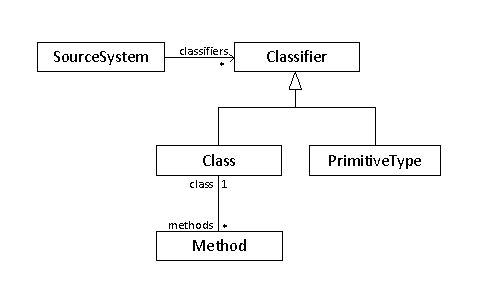
\includegraphics[scale=0.7]{figures/sourceMetamodel}
\caption{Source meta-model}
\label{fig:sourceMetamodel}
\end{minipage}
\hfill
\begin{minipage}[b]{0.55\linewidth}
\centering
	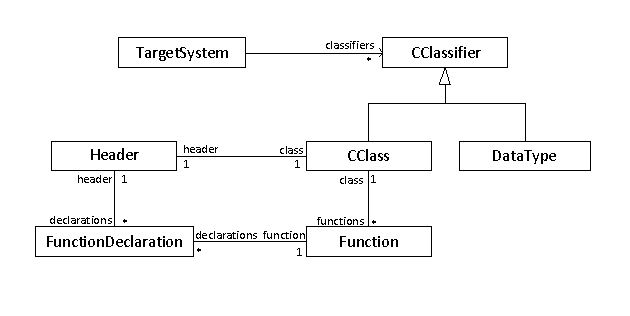
\includegraphics[scale=0.7]{figures/targetMetamodel}
\caption{Target meta-model}
\label{fig:targetMetamodel}
\end{minipage}

\end{figure}


Figure~\ref{fig:sourceMetamodel} shows a simplified meta-model for an ASG which acts as the source meta-model for our exemplary transformation scenario. A \fe{SourceSystem} consists of a number of \fe{Classifiers} which can either be \fe{PrimitiveTypes} or \fe{Classes}. Each \fe{Class} can have a number of \fe{Methods}.

The target meta-model for the transformation, shown in Figure~\ref{fig:targetMetamodel}, is slightly more complex.
The \fe{TargetSystem} consists of a number of \fe{CClassifiers} which are either \fe{DataTypes} or \fe{CClasses}.
An \fe{CClass} can contain a number of \fe{Functions}. In addition, each \fe{CClass} has a corresponding \fe{Header} which contains a \fe{FunctionDeclaration} for each \fe{Function} of the \fe{CClass}.


\begin{figure}[htbp]
\begin{center}
  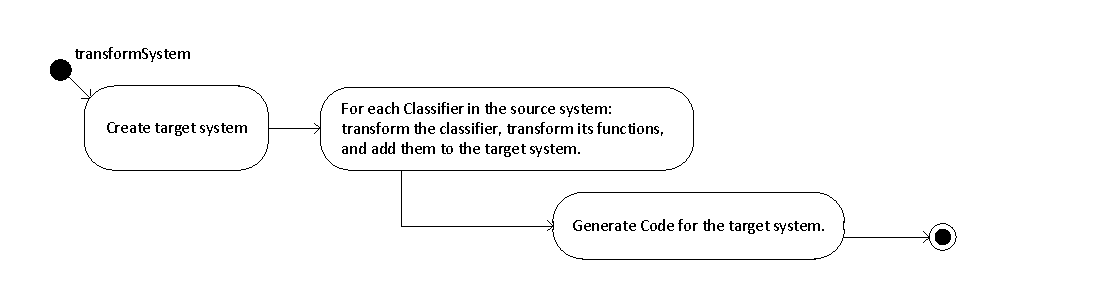
\includegraphics[width=\textwidth]{figures/transformationOverview}
  \caption{An activity diagram describing the example transformation}
  \label{fig:transformationOverview}
\end{center}
\end{figure}

Figure~\ref{fig:transformationOverview} shows an activity diagram which gives an overview of the transformation from a source ASG to a target ASG.
At first, the target system has to be created. Each classifier in the source system has to be transformed into a corresponding classifier in the target system. While primitive types can be transformed easily, headers have to be created for all transformed classes. For each method, a function has to be created and a corresponding function declaration has to be added to the correct header. In the end, the target system can be passed to the code generation mechanism.

\subsection{Requirements}

Vorschlag fuer das Beispiel: Interface Violation Reengineering Beispiel, die Konstrukte (x) sind bereits enthalten, die Konstrukte (...) sind Ideen, wie man das Beispiel ergaenzen kann

Das Beispiel muss enthalten:
\begin{itemize}
  \item Komplexer Kontrollfluss (success und failure (x), forEach (x), exception und finally, boolean conditions), verschiedene Node Types (normal (x), forEach (x), start (x), stop (x), Junction)
  \item StatementNode und TextualExpression (wollen wir eigentlich nicht)
  \item Negative Anwendungsbedingung (x) und komplexe negative Anwendungsbedingung (Subpattern eines Story Pattern) (kann im Beispiel ergaenzt werden, indem man in Activity 6 prueft, ob die Klasse nicht eine andere Methode mit dem gleichen Namen und Rueckgabetyp enthaelt) 
  \item Calls inkl. polymorphic dispatching  (evtl. Activities 6-8 rausziehen und ueber call aufrufen)
  \item Expressions (Attribute Assigments (x), Attributvergleich beim Matching (x), Constraint eines Story Pattern (evtl. in Activity 5 oder Activity 6 class != acessedMethodOwner einfuegen)), LinkConstraints (z.B. neue Methode als letzte in die Liste einsortieren, neue Methode in alphabetischer Reihenfolge einsortieren)
  \item SetObjects, Links zum Zugreifen eines Sets und Constraints fuer diese (Zaehlen wie viele Klassen das Interface implementieren, oder Activity 5 ueber ein Set Object loesen)
  \item Structured Nodes und Flow Stops
  \item Pattern Matching: Optional, Maybe bound, Optional create, Optional destroy? (Evtl. zusaetzliche Story Diagramme addSuperClass, removeSuperClass bei denen fuer alle Methoden Overrides ergaenzt bzw. geloescht)
  \item Maybe construct, um Isomorphietest fuer zwei gebundene Objekte zu deaktivieren
  \item Templates (evtl. Beispiel fuer anderen AST oder Ecore/UML generalisieren)
\end{itemize}